\documentclass[12pt, oneside]{article}

\usepackage[letterpaper, scale=0.89, centering]{geometry}
\usepackage{fancyhdr}
\setlength{\parindent}{0em}
\setlength{\parskip}{1em}

\pagestyle{fancy}
\fancyhf{}
\renewcommand{\headrulewidth}{0pt}
\rfoot{\href{https://creativecommons.org/licenses/by-nc-sa/2.0/}{CC BY-NC-SA 2.0} Version \today~(\thepage)}

\usepackage{amssymb,amsmath,pifont,amsfonts,comment,enumerate,enumitem}
\usepackage{currfile,xstring,hyperref,tabularx,graphicx,wasysym}
\usepackage[labelformat=empty]{caption}
\usepackage[dvipsnames,table]{xcolor}
\usepackage{multicol,multirow,array,listings,tabularx,lastpage,textcomp,booktabs}

\lstnewenvironment{algorithm}[1][] {   
    \lstset{ mathescape=true,
        frame=tB,
        numbers=left, 
        numberstyle=\tiny,
        basicstyle=\rmfamily\scriptsize, 
        keywordstyle=\color{black}\bfseries,
        keywords={,procedure, div, for, to, input, output, return, datatype, function, in, if, else, foreach, while, begin, end, }
        numbers=left,
        xleftmargin=.04\textwidth,
        #1
    }
}
{}
\lstnewenvironment{java}[1][]
{   
    \lstset{
        language=java,
        mathescape=true,
        frame=tB,
        numbers=left, 
        numberstyle=\tiny,
        basicstyle=\ttfamily\scriptsize, 
        keywordstyle=\color{black}\bfseries,
        keywords={, int, double, for, return, if, else, while, }
        numbers=left,
        xleftmargin=.04\textwidth,
        #1
    }
}
{}

\newcommand\abs[1]{\lvert~#1~\rvert}
\newcommand{\st}{\mid}

\newcommand{\A}[0]{\texttt{A}}
\newcommand{\C}[0]{\texttt{C}}
\newcommand{\G}[0]{\texttt{G}}
\newcommand{\U}[0]{\texttt{U}}

\newcommand{\cmark}{\ding{51}}
\newcommand{\xmark}{\ding{55}}

 
\begin{document}
\begin{flushright}
    \StrBefore{\currfilename}{.}
\end{flushright} 
\section*{Monday October 11}


{\bf Logical operators} aka propositional connectives

\begin{tabular}{lccccp{4in}}
{\bf Conjunction} & AND & $\land$ &\verb|\land| & 2 inputs & Evaluates to $T$ exactly when {\bf both} inputs are $T$\\
{\bf Exclusive or} & XOR & $\oplus$ &\verb|\oplus| & 2 inputs & Evaluates to $T$ exactly when {\bf exactly one} of inputs is $T$\\
{\bf Disjunction} & OR & $\lor$ &\verb|\lor| & 2 inputs & Evaluates to $T$ exactly when {\bf at least one} of inputs is $T$\\
{\bf Negation} & NOT & $\lnot$ &\verb|\lnot| & 1 input & Evaluates to $T$ exactly when its input is $F$\\
\end{tabular} 

\begin{center}
\begin{tabular}{cc||c|c|c}
\multicolumn{2}{c||}{Input}  & \multicolumn{3}{c}{Output} \\
& & {\bf Conjunction} &  {\bf Exclusive or} & {\bf Disjunction} \\
$p$ & $q$ & $p \land q$ &  $p  \oplus  q$ & $p \lor  q$ \\
\hline
$T$ & $T$ & $T$ & $F$ & $T$\\
$T$ & $F$ & $F$ & $T$ & $T$\\
$F$ & $T$ & $F$ & $T$ & $T$\\
$F$ & $F$ & $F$ & $F$ & $F$\\
\hline
& & \includegraphics[width=0.5in]{../../resources/images/xANDy.png}
&  \includegraphics[width=0.5in]{../../resources/images/xXORy.png}
&  \includegraphics[width=0.5in]{../../resources/images/xORy.png}
\end{tabular}
\qquad \qquad\qquad
\begin{tabular}{c||c}
Input & Output \\
& {\bf Negation} \\
$p$ & $\lnot p$ \\
\hline
$T$ & $F$ \\
$F$ & $T$\\
\hline & 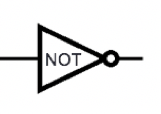
\includegraphics[width=0.5in]{../../resources/images/NOTx.png}
\end{tabular}
\end{center}
 

\begin{center}
    \begin{tabular}{ccc||p{3in}|c|c}
    \multicolumn{3}{c||}{Input}  & \multicolumn{3}{c}{Output} \\
    $p$ & $q$ & $r$  &  &  $(p \land q) \oplus (~ ( p \oplus q) \land r~)$ & $(p \land q) \vee (~ ( p \oplus q) \land r~)$ \\
    \hline
    $T$ & $T$  & $T$ &   && \\
    $T$ & $T$  & $F$ &   && \\
    $T$ & $F$  & $T$ &   && \\
    $T$ & $F$  & $F$ &   && \\
    $F$ & $T$  & $T$ &   && \\
    $F$ & $T$  & $F$ &   && \\
    $F$ & $F$  & $T$ &   && \\
    $F$ & $F$  & $F$ &   && \\
    \end{tabular}
\end{center}
    \vfill \newpage


Given a truth table, how do we find an expression
using the input variables and logical operators that has the 
output values specified in this table?

{\it Application}: design a circuit given a desired input-output relationship.

\begin{center}
\begin{tabular}{cc||cc}
\multicolumn{2}{c||}{Input}  &\multicolumn{2}{c}{Output}\\
$p$ & $q$& $mystery_1$ & $mystery_2$\\
\hline
$T$ & $T$  & $T$ & $F$\\
$T$ & $F$  & $T$ & $F$\\
$F$ & $T$  & $F$ & $F$\\
$F$ & $F$  & $T$ & $T$\\
\end{tabular}
\end{center}


Expressions that have output $mystery_1$ are

\vspace{100pt}

Expressions that have output $mystery_2$ are

\vspace{100pt}
 

{\bf  Definition} An expression built of variables and logical 
operators is in {\bf disjunctive normal form}  (DNF) means
that it is an OR of ANDs of variables and their negations.

{\bf  Definition} An expression built of variables and logical 
operators is in {\bf conjunctive normal form}  (CNF) means
that it is an AND of ORs of variables and their negations.
 



{\it Extra example}: An expression that has output ? is: 

\begin{tabular}{ccc||c}
    \multicolumn{3}{c||}{Input}  & Output\\
    $p$ & $q$ & $r$  &  ?\\
    \hline
    $T$ & $T$  & $T$ & $T$ \\
    $T$ & $T$  & $F$ & $T$ \\
    $T$ & $F$  & $T$ & $F$ \\
    $T$ & $F$  & $F$ & $T$ \\
    $F$ & $T$  & $T$ & $F$ \\
    $F$ & $T$  & $F$ & $F$ \\
    $F$ & $F$  & $T$ & $T$ \\
    $F$ & $F$  & $F$ & $F$ \\
\end{tabular}

\vfill

 \newpage


{\bf Proposition}: Declarative sentence that is true or false (not both).

{\bf Propositional variable}: Variable that represents a proposition.

{\bf Compound proposition}: New proposition formed from existing propositions (potentially) using logical operators.
{\it Note}: A propositional variable is one example of a compound proposition.

{\bf Truth table}: Table with one row for each of the possible combinations of truth values of the input and 
    an additional column that shows the truth value of the result of the operation corresponding to a particular row.
    
 

{\bf Logical equivalence }: Two compound  propositions are {\bf logically  equivalent} means that  they 
have the  same  truth  values for all settings of truth  values to their propositional  variables.

{\bf Tautology}:  A compound proposition that evaluates to true
for all settings of truth  values to its propositional  variables; it is  abbreviated $T$.

{\bf Contradiction}: A compound proposition that  evaluates  to  false 
for  all settings of truth  values to its propositional  variables; it  is abbreviated $F$.

{\bf Contingency}: A compound proposition that is neither a tautology nor a contradiction.
 \vfill


Label each of the following as a tautology, contradiction, or contingency.

$p \land p$

$p \oplus p$

$p \lor p$

$p \lor \lnot p$

$p \land \lnot p$ \vfill


{\it Extra Example}: Which of the  compound propositions in the table below are logically equivalent?
\begin{center}
\begin{tabular}{cc||c|c|c|c|c}
\multicolumn{2}{c||}{Input}  & \multicolumn{5}{c}{Output} \\
$p$ & $q$ & $\lnot (p \land \lnot q)$ & $\lnot (\lnot p  \lor \lnot q)$ &  $(\lnot p \lor  q)$
& $(\lnot q \lor \lnot p)$ & $(p \land q)$  \\
\hline
$T$ & $T$ & &&&&\\
$T$ & $F$ & &&&&\\
$F$ & $T$ & &&&&\\
$F$ & $F$ & &&&&\\
\end{tabular}
\end{center} \vfill
\newpage
\subsection*{Review: Week 3 Monday}
\begin{enumerate}
    \item 

\begin{enumerate}
    \item Consider the logic circuit
    \begin{center}
    \includegraphics[width=2in]{../../resources/images/review-circuit-3.png}
    \end{center}
    For which of the following settings(s) of input values is the output
    $y_1 =  0$? (Select all and only those that apply.)
    \begin{enumerate}
        \item $x_1 = 0$, $x_2 = 0$, $x_3 = 0$, and $x_4 = 0$
        \item $x_1 = 1$, $x_2 = 1$, $x_3 = 1$, and $x_4 = 1$
        \item $x_1 = 1$, $x_2 = 0$, $x_3 = 0$, and $x_4 = 1$
        \item $x_1 = 0$, $x_2 = 0$, $x_3 = 1$, and $x_4 = 1$
    \end{enumerate}
    \item Consider the logic circuits
    \begin{center}
    \includegraphics[width=2in]{../../resources/images/review-circuit-1.png}
    \qquad \qquad \qquad
    \includegraphics[width=2in]{../../resources/images/review-circuit-4.png}
    \end{center}
    For which  of the following settings(s) of input values do the outputs
    of these  circuits have the  same value, i.e.\ $y_1 =  z_1$? 
    (Select all and only those that apply.)
    \begin{enumerate}
        \item $x_1 = 1$, $x_2 = 1$
        \item $x_1 = 1$, $x_2 = 0$
        \item $x_1 = 0$, $x_2 = 1$
        \item $x_1 = 0$, $x_2 = 0$
    \end{enumerate}    
    
\end{enumerate}     \item 

For each of the following compound propositions, determine
if it is in DNF, CNF, both, or neither.

\begin{enumerate}
    \item $(x \lor y \lor z) \land (x \land \lnot y \land z)$
    \item $\lnot (x \land y \land z) \land \lnot (\lnot x \land y \land \lnot z)$
\end{enumerate} \end{enumerate}
\newpage
\section*{Wednesday October 13}


\begin{center}
    \begin{tabular}{cc||c|c|c|c|c}
    \multicolumn{2}{c||}{Input}  & \multicolumn{5}{c}{Output} \\
     & & Conjunction &  Exclusive or & Disjunction  &  Conditional & Biconditional  \\
    $p$ & $q$ & $p \wedge q$ &  $p  \oplus  q$ & $p \vee  q$ & $p \to q$ & $p \leftrightarrow q$\\
    \hline
    $T$ & $T$ & $T$ & $F$ & $T$ & $T$& $T$\\
    $T$ & $F$ & $F$ & $T$ & $T$ & $F$& $F$\\
    $F$ & $T$ & $F$ & $T$ & $T$ & $T$& $F$\\
    $F$ & $F$ & $F$ & $F$ & $F$ & $T$& $T$\\
    \hline
    && ``$p$ and $q$'' & ``$p$ xor $q$'' & ``$p$ or $q$'' & ``if $p$ then $q$'' & ``$p$ if and only if $q$''
    \end{tabular}
\end{center}
     

The only way to make  the conditional statement $p \to q$ false is to \underline{\phantom{\hspace{3in}}}\\

\begin{tabular}{llll}
The {\bf  hypothesis}  of $p \to q$ is  &\underline{\phantom{\hspace{1in}}} &
The {\bf  antecedent}  of $p \to q$ is  &\underline{\phantom{\hspace{1in}}} \\
&&&  \\
The {\bf  conclusion}  of $p \to q$ is & \underline{\phantom{\hspace{1in}}}&
The {\bf  consequent}  of $p \to q$ is & \underline{\phantom{\hspace{1in}}}\\
&&&  \\
\end{tabular}
 

The {\bf converse}  of $p \to q$ is \underline{\phantom{ $q \to p$\hspace{1.6in}}}\\

The {\bf inverse}  of $p \to q$ is \underline{\phantom{ $\lnot p \to \lnot q$\hspace{1.6in}}}\\

The {\bf contrapositive}  of $p \to q$ is \underline{\phantom{$\lnot q \to \lnot p$\hspace{1.6in}}} \\
 \vfill


Order of operations (Precedence) for logical operators: 

Negation, then conjunction / disjunction, then conditional / biconditionals.

Example: $\lnot p \lor \lnot q$ means $(\lnot p) \lor (\lnot q)$.
 \newpage


{\bf (Some) logical equivalences}

{\it Can replace $p$ and $q$ with any compound proposition}

\begin{tabular}{llp{3in}}
$\lnot ( \lnot p) \equiv p$ & & {\bf Double negation}\\
&& \\
&& \\
$p \lor q \equiv q \lor p$ & $p \land q \equiv q \land p$ & {\bf Commutativity} Ordering of terms\\
&& \\
&& \\
$(p \lor q) \lor r  \equiv p \lor (q \lor r)$ & $(p \land q) \land r  \equiv p \land (q \land r)$ & {\bf Associativity} Grouping of terms\\
&& \\
&& \\
$p \land F \equiv F$ \qquad $p \lor T \equiv T$ & $p \land T \equiv p$ \qquad $p \lor F \equiv p$ & {\bf Domination} aka 
short circuit evaluation\\
&& \\
&& \\
$\lnot (p \land q) \equiv \lnot p \lor \lnot q$ & $\lnot (p \lor q) \equiv \lnot p \land\lnot q$  & {\bf DeMorgan's Laws}\\
&& \\
\end{tabular}

\begin{tabular}{llp{3in}}
$p \to q \equiv \lnot p \lor q$ & & \\
&& \\
&& \\
$p \to q \equiv \lnot q \to \lnot p$ & &{\bf Contrapositive} \\
&& \\
&& \\
$\lnot (p \to q) \equiv p\land \lnot q$  & &\\
&& \\
&& \\
$\lnot( p \leftrightarrow q) \equiv p \oplus q$ && \\
&& \\
&& \\
$p \leftrightarrow q \equiv q \leftrightarrow p$ &&\\
&& \\
\end{tabular}

{\it Extra examples}:

$p \leftrightarrow q$ is not logically equivalent to $p \land q$ because \underline{\phantom{\hspace{4in}}} 

$p \to q$ is not logically equivalent to $q \to p$ because \underline{\phantom{\hspace{4in}}} 
 \newpage


{\bf Common ways to express logical operators in English}:

{\bf Negation} $\lnot p$ can be said in English as 
\begin{itemize}
\item Not $p$.
\item It's not the case that $p$.
\item $p$ is false.
\end{itemize}

{\bf Conjunction} $p \land q$ can be said in English as
\begin{itemize}
    \item $p$ and $q$.
    \item Both $p$ and $q$ are true.
    \item $p$ but $q$.
\end{itemize}

{\bf Exclusive or} $p \oplus q$ can be said in English as
\begin{itemize}
    \item $p$ or $q$, but not both.
    \item Exactly one of $p$ and $q$ is true.
\end{itemize}

{\bf Disjunction} $p \lor q$ can be said in English as
\begin{itemize}
    \item $p$ or $q$, or both.
    \item $p$ or $q$ (inclusive).
    \item At least one of $p$ and $q$ is true.
\end{itemize}

{\bf Conditional} $p \to q$ can be said in English as
\begin{multicols}{2}
\begin{itemize}
    \item if $p$, then $q$.
    \item $p$ is sufficient for $q$.
    \item $q$ when $p$.
    \item $q$ whenever $p$.
    \item $p$ implies $q$.
    \item $q$ follows from $p$.
    \item $p$ is sufficient for $q$.
    \item $q$ is necessary for $p$.
    \item $p$ only if $q$.
\end{itemize}
\end{multicols}

{\bf Biconditional}
\begin{itemize}
    \item $p$ if and only if $q$.
    \item $p$ iff $q$.
    \item If $p$ then $q$, and conversely.
    \item $p$ is necessary and sufficient for $q$.
\end{itemize} \newpage
\subsection*{Review: Week 3 Wednesday}
\begin{enumerate}
    \item 

For each of the following propositions, indicate exactly one of:

\begin{itemize}
    \item There is no assignment of truth values to its variables that makes it true,
    \item There is exactly one assignment of truth values to its variables that makes it true, or
    \item There are exactly two assignments of truth values to its variables that make it true, or
    \item There are exactly three assignments of truth values to its variables that make it true, or
    \item \emph{All} assignments of truth values to its variables make it true.
\end{itemize}

\begin{enumerate}
    \item $x \land y \land (x \lor y)$
    \item $\lnot x \land y \land (x \lor y)$
    \item $x \land \lnot y \land (x \land y)$
    \item $\lnot x \land (y \lor \lnot y)$
    \item $x \land (y \lor \lnot x)$
\end{enumerate}     \item 

For each of the following propositions, indicate exactly one of:

\begin{itemize}
    \item There is no assignment of truth values to its variables that makes it true,
    \item There is exactly one assignment of truth values to its variables that makes it true, or
    \item There are exactly two assignments of truth values to its variables that make it true, or
    \item There are exactly three assignments of truth values to its variables that make it true, or
    \item \emph{All} assignments of truth values to its variables make it true.
\end{itemize}

\begin{enumerate}
    \item $(p \leftrightarrow q) \oplus (p \land q)$
    \item $(p \to q) \vee (q \to p)$
    \item $(p \to q) \land (q \to p)$
    \item $\lnot (p \to q) $
\end{enumerate} \end{enumerate}
\newpage
\section*{Friday October 15}


We can use a recursive definition to describe all 
compound propositions that use propositional variables 
from a specified collection.  Here's the definition
for all compound propositions whose propositional variables 
are in $\{p, q\}$.

\[
\begin{array}{ll}
\textrm{Basis Step: } & p \textrm{ and } q \textrm{ are each a compound proposition} \\
\textrm{Recursive Step: } & \textrm{If } x \textrm{ is a compound proposition then so is } (\lnot x) 
\textrm{ and if } \\
& x \textrm{ and } y \textrm{ are both compound propositions then so is each of }\\
&(x \land y), (x \oplus y), (x \lor y), (x \to y), (x \leftrightarrow y)
\end{array}
\] \newpage


{\bf Translation}: Express each of the following sentences as compound propositions, using
the given propositions.

\begin{multicols}{2}
``A sufficient condition for the warranty to be good is that you bought the computer less than a year ago"
\columnbreak
\begin{align*}
w &\text{ is  ``the warranty is good"} \\
b &\text{ is  ``you bought the computer less than a year ago"} \\
\end{align*}
\end{multicols}
\vfill

\begin{multicols}{2}
``Whenever the message was sent from an unknown system, it is scanned for viruses."
\columnbreak
\begin{align*}
s &\text{ is  ``The message is scanned for viruses"} \\
u &\text{ is  ``The message was sent from an unknown system"} \\
\end{align*}
\end{multicols}
\vfill

\begin{multicols}{2}
``I will complete my to-do list only if I put a reminder in my calendar"
\columnbreak
\begin{align*}
d &\text{ is  ``I will complete my to-do list"} \\
c &\text{ is  ``I put a reminder in my calendar"} \\
\end{align*}
\end{multicols}
\vfill \newpage


{\bf Definition}: A collection of  compound  propositions
is called {\bf consistent} if  there
is  an assignment  of  truth values
to  the  propositional variables that makes
each of the compound propositions  true.
 

{\bf Consistency}: 
\begin{quote}
Whenever the system software is being upgraded, users cannot access the file system. 
If users can access the file system, then they can save new files. 
If users cannot save new files, then the system software is not being upgraded.
\end{quote}

\begin{enumerate}
\item Translate to symbolic compound propositions
\vfill
\item Look for some truth assignment to the propositional variables for which all the compound propositions output $T$
\vfill
\end{enumerate} \newpage
\subsection*{Review: Week 3 Friday}
\begin{enumerate}
    \item 

Express each of the following sentences as compound propositions, using
the given propositions.

\begin{enumerate}
\item ``If you try to run Zoom while your computer is running many applications,
the video is likely to be choppy and laggy." $t$ is ``you run Zoom while your
computer is running many applications'', $c$ is ``the video is likely to be choppy'',
$g$ is ``the video is likely to be laggy''
\begin{enumerate}
    \item $t \to (c \land g)$
    \item $(c \land g) \to t$
    \item $(c \land g) \leftrightarrow t$
    \item $t \oplus (c \land g)$
\end{enumerate}
\item ``To connect wirelessly on campus without logging in you need to use
the UCSD-Guest network."  $c$ is ``connect wirelessly 
on campus'', $g$ is ``logging in'', and $u$ is ``use UCSD-Guest network''.
\begin{enumerate}
    \item $c \land \lnot g \land u$
    \item $(c \land \lnot g) \lor u$
    \item $(c \land \lnot g) \oplus u$
    \item $(c \land \lnot g) \to u$
    \item $u \to (c \land \lnot g)$
    \item $u \leftrightarrow (c \land \lnot g)$
\end{enumerate}
\end{enumerate}
\vspace{20pt}     \item 

For each of  the following  system specifications, 
identify the compound propositions  that give their
translations to logic  and then determine if the
translated collection  of compound
propositions is consistent.

\begin{enumerate}
    \item Specification: If the computer is out of memory, then network connectivity is unreliable. No disk errors can occur when the computer is out of memory. Disk
    errors only occur when network connectivity is unreliable.
    
    Translation: $M =$ ``the computer is  out of memory"; $N = $ ``network connectivity
    is unreliable"; $D = $  ``disk errors  can occur".
    
    \begin{enumerate}
        \item \begin{align*} &\neg M \to  N  \\ & \neg D \to M \\ & D \to N \end{align*}
        \item \begin{align*} &M \to  \neg N  \\ & \neg D \wedge M \\ & N \to D \end{align*}
        \item \begin{align*} &M \to  N  \\ &  M \to \neg D \\ & \neg  N \to \neg D \end{align*}
    \end{enumerate}
    
    \newpage
    \item Specification: Whether you think you can, or you think you can't - you're right.
\footnote{Henry Ford}
    
    Translation: $T =$ ``you  think  you  can"; $C = $  ``you  can".
    
    \begin{enumerate}
        \item \begin{align*} &T \to C \\&  \neg T \to \neg C \end{align*}
        \item \begin{align*} &T \wedge C \\  & \neg  T \wedge \neg C \end{align*}
        \item \begin{align*} &T \to \neg T  \\ & C  \to \neg  C \end{align*}
    \end{enumerate}
    
    \item Specification: A secure password must be private and complicated. If
    a password is  complicated then  it will be hard to  remember.  People
    write down hard-to-remember passwords. If a password is written down, it's  not private.   The password is secure.

    Translation: $S =$ ``the password is secure"; $P = $ ``the password is private"; 
    $C = $  ``the password is  complicated"; $H = $ ``the password is hard to remember";
    $W =  $ ``the password is written down".
    
    \begin{enumerate}
        \item \begin{align*} &\neg (P \wedge C) \to \neg  S  \\ & C \to H  \\ & W \wedge H \\ & W \to  \neg P \\ & S \end{align*}
        \item \begin{align*} &(P \wedge  C)  \to S  \\ &  C \to H\\ & W  \to  H \\  & W \to P \\ & S\end{align*}
        \item \begin{align*} & S  \to (P \wedge C)  \\ &  C \to H\\ & H  \to  W \\  & W \to \neg P \\ & S\end{align*}
    \end{enumerate}

\end{enumerate} \end{enumerate}
\end{document}
